%!TEX root = ../../../main.tex

\section{Kripke structures}

% ---------------------------------------------------------------------

\begin{frame}{System model}

We shall use a very generic (and unspecific) model, i.e.
  \hl{transition systems}, essentially directed graphs:

\begin{equation*}
  {\cal T}=(S,\mathord{\to},r)
\end{equation*}
  
\bigskip
 $\mathbf{S}\qquad\qquad\qquad\>\>\>\widehat=\qquad$
  \hl{state space}; 
  \\ \vspace{.1cm}\quad\quad {\small states that the system may attain (finite or infinite set)}

  \bigskip
 $\mathbf{\mathord{\to}\subseteq S\times S}\qquad\>\widehat=\qquad$
   \hl{transition relation}; 
   \\ \vspace{.1cm}\quad\quad {\small describes which actions or ``steps'' are possible}
  
  \bigskip
 $\mathbf{r\in S}\qquad\qquad\,\ \ \ \widehat=\qquad$
    \hl{initial state} (``root'')

\end{frame}


% ---------------------------------------------------------------------

\begin{frame}{Example 1: Producer/Consumer}

(Pseudocode) program with variables and concurrency:

\bigskip
$\mbox{{\bf var} \  {\it turn} \  \{0,1\} \  {\bf init} \  0;}$\\
$\mbox{{\bf cobegin} } \:\{ \tc{blue}{P} \parallel \tc{magenta}{K} \} \: \mbox{ {\bf coend}}$


\bigskip
$\tc{blue}{P} = $ \tc{blue}{%\hspace{.1cm}
\begin{minipage}[t]{4cm}
\begin{tabbing}
colu \= co \= colu \= \kill
{\bf start}; \\
{\bf while} {\bf true} {\bf do} \\
\> $w_0$: \> {\bf wait} $({\it turn} = 0)$; \\
\> $p_0$: \> /* produce */ \\
\>        \> ${\it turn} := 1$; \\
{\bf od};\\
{\bf end}
\end{tabbing}
\end{minipage}}
%\hspace{.5cm}
$\tc{magenta}{K} = $ \tc{magenta}{%\hspace{.01cm}
\begin{minipage}[t]{4cm}
\begin{tabbing}
colu \= co \= colu \= \kill
{\bf start}; \\
{\bf while} {\bf true} {\bf do} \\
\> $w_1$: \> {\bf wait} $({\it turn} = 1)$; \\
\> $c_1$: \> /* consume */ \\
\>        \> ${\it turn} := 0$; \\
{\bf od};\\
{\bf end}
\end{tabbing}
\end{minipage}}
\end{frame}


% ---------------------------------------------------------------------

\begin{frame}{Example 1: Corresponding transition system}

$S = \tc{blue}{\{w_0,p_0\}}\times\tc{magenta}{\{w_1,c_1\}}\times\{0,1\}$;
  \quad Initial state: $(w_0,w_1,0)$

\bigskip
\begin{center}
  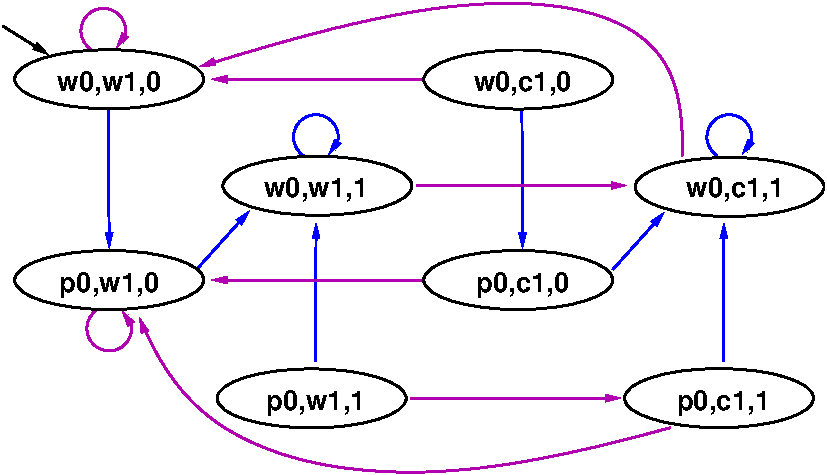
\includegraphics[width=\textwidth]{content/chapter_model_checking/model_checking/images/mutex-ts}
\end{center}

\end{frame}


% ---------------------------------------------------------------------
\begin{frame}{Example 2: Petri net}

State space = set of markings\\[1cm]

\setlength{\unitlength}{.025\textwidth}\hfil%
\begin{picture}(18,12.5)(0,0)
%place and transition symbols
\multiput(1,3)(8,0){3}{\circle2}\multiput(4,2)(8,0){2}{\framebox(2,2){}}
\multiput(1,9.5)(8,0){2}{\circle2}\put(4,8.5){\framebox(2,2){}}
% place labels
\put(0,0){\makebox(2,1.5)[t]{\blue{$p_1$}}}
\put(8,0){\makebox(2,1.5)[t]{\blue{$p_3$}}}
\put(16,0){\makebox(2,1.5)[t]{\blue{$p_5$}}}
\put(0,11){\makebox(2,1.5)[b]{\blue{$p_2$}}}
\put(8,11){\makebox(2,1.5)[b]{\blue{$p_4$}}}
% transition labels
\put(4,0){\makebox(2,1.5)[t]{\blue{\small$t_1$}}}
\put(12,0){\makebox(2,1.5)[t]{\blue{\small$t_3$}}}
\put(4,11){\makebox(2,1.5)[b]{\blue{\small$t_2$}}}
% initial marking
\multiput(1,3)(0,6.5){2}{\circle*{.5}}
% arcs
\multiput(2,3)(4,0){4}{\vector(1,0){2}}
\multiput(2,9.5)(4,0){2}{\vector(1,0){2}}
\put(7,8.5){\oval(12,4.5)[lb]}\put(7,4){\oval(12,4.5)[rt]}
\put(13,4){\vector(0,-1){0}}
\end{picture}\hfil%
\setlength{\unitlength}{.025\textwidth}\hfil%
\begin{picture}(16,12.5)(0,0)
% transitions
\multiput(6,1.5)(-4,5.5){2}{\vector(1,1){4}}
\multiput(8,1.5)(-4,5.5){2}{\makebox(2,2)[lt]{\blue{\small$t_1$}}}
\multiput(6,1.5)(4,5.5){2}{\vector(-1,1){4}}
\multiput(2,1.5)(4,5.5){2}{\makebox(2,2)[rt]{\blue{\small$t_2$}}}
\put(10,7){\vector(1,1){4}}\put(12,7){\makebox(2,2)[lt]{\blue{\small$t_3$}}}
% markings
\put(4,0){\makebox(4,1.5){$\to$\ \blue{$\tuple{1\!,1\!,0\!,0\!,0}$}}}
\put(0,5.5){\makebox(4,1.5){\blue{$\tuple{1\!,0\!,0\!,1\!,0}$}}}
\put(8,5.5){\makebox(4,1.5){\blue{$\tuple{0\!,1\!,1\!,0\!,0}$}}}
\put(4,11){\makebox(4,1.5){\blue{$\tuple{0\!,0\!,1\!,1\!,0}$}}}
\put(12,11){\makebox(4,1.5){\blue{$\tuple{0\!,0\!,0\!,0\!,1}$}}}
\end{picture}\hfil
\end{frame}

% ---------------------------------------------------------------------

\begin{frame}{Implicitly given transition systems}
\begin{itemize}
\itemsep1em
\item Quite often, a transition system is given to us ``implicitly'',
   i.e.\ in the form of a program, from which we extract the
   transition system.

\item In such a setting, we are given an initial state and a function
   for computing the direct successor states of a given state, such that
   transitions are computed only on demand.

\item Some of our analysis methods will be suitable for such a setting.
\end{itemize}
\end{frame}

% ----------------------------------------------------------------------

\begin{frame}{Finite and infinite transition systems}

In principle, a transition system many have infinitely many states.
Some of the possible reasons are:
\bigskip

\begin{itemize}
\item \hl{Data:} integers, reals, lists, trees, pointer structures, \ldots
\item \hl{Control:} (recursive) procedures, dynamic thread creation, \ldots
\item \hl{Communication:} unbounded FIFO channels, \ldots
\item \hl{Unknown parameters}: number of participants in a protocol, \ldots
\item \hl{Real time}: discrete or continuous time
\end{itemize}

\bigskip
 Some (not all!) of these features lead to \red{Turing-powerful}
 computation models (and thus \red{undecidable}
 verification problems).

\end{frame}

% ----------------------------------------------------------------------

\begin{frame}{Example: Petri net}
Petri nets may have an infinite state space, too:

\bigskip
\begin{center}
{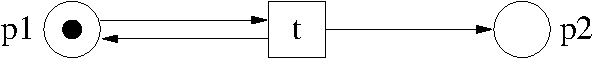
\includegraphics[width=\textwidth]{content/chapter_model_checking/model_checking/images/infinite}}
\end{center}

\bigskip
Reachable states are:
\blue{$\tuple{1,0},\ \tuple{1,1},\ \tuple{1,2},\ \ldots$}

\bigskip
Reachability and LTL decidable, CTL undecidable.

\end{frame}

% ---------------------------------------------------------------------

\begin{frame}{Finite Kripke structures}
\begin{itemize}
\itemsep1em
\item For now, we restrict ourselves to finite state spaces.

\item Finite systems: e.g.\ hardware systems, programs with finite
   data typs (Boolean programs), certain communication protocols, \ldots

\item Finite systems may also be obtained by \hl{abstracting} an
   infinite system.

\item Remaining problem: \red{state-space explosion},
   systems may be finite but VERY large.   
\end{itemize}
\end{frame}

% ---------------------------------------------------------------------

\begin{frame}{Reasons for state-space explosion (1)}

A common reason is \hl{concurrency}.

\bigskip
\hl{Example}: Consider the following Petri net:

\bigskip
\begin{center}
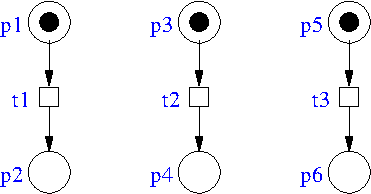
\includegraphics[width=.8\textwidth]{content/chapter_model_checking/model_checking/images/3prozesse}
\end{center}

\end{frame}

% ---------------------------------------------------------------------

\begin{frame}{}

The reachability graph has got \blue{$8=2^3$} states and \blue{$6=3!$}
paths.

\bigskip
\begin{center}
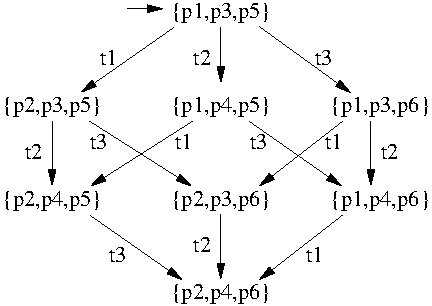
\includegraphics[width=.8\textwidth]{content/chapter_model_checking/model_checking/images/3pkrip}
\end{center}

\bigskip
With \blue{$n$} components we have \blue{$2^n$} states and \blue{$n!$} paths.

\end{frame}

% ---------------------------------------------------------------------

\begin{frame}{Reasons for state-space explosion (2)}

A second common reason is \hl{data}.
\begin{itemize}
  \item e.g.\ programs with few large or many small variables
  \item size of state space: 2 to the number of bits
\end{itemize}

\bigskip
Counteractions:
\begin{itemize}
\item \hl{Abstraction}: ignore ``unimportant'' data
\item \hl{Compression}: work with \emph{sets} of states;
  efficient data structures for storing and manipulating sets
\item \hl{Approximation}: find over- or underapproximations of the
  reachable states
\end{itemize}

\end{frame}

% ---------------------------------------------------------------------

\begin{frame}{Kripke structures}

Idea: Extract from each state a \hl{valuation}.
\begin{center}
$${\cal K} = (S,\mathord{\to},r,AP,\nu)$$
\end{center}

\begin{align*}
(S,\mathord{\to},r) \quad \widehat= \quad  &
   \text{underlying \hl{transition system}} \\
AP \quad  \widehat= \quad &
   \text{set of \hl{atomic propositions}} \\
\nu\colon S \to 2^{AP} \quad  \widehat= \quad &
   \text{\hl{interpretation} of atomic propositions} \\
& \text{(``valuation'')}
\end{align*}

\bigskip 
Remarks:
\begin{itemize}
\item $2^{AP}$ denotes the \emph{powerset} of $AP$.
\item Valuations are represented here as subsets of \m{AP} rather
   than functions; the propositions contained in the set are
   those that are deemed true.
\end{itemize}
\end{frame}

% ---------------------------------------------------------------------

\begin{frame}{Example of a Kripke structure}
\begin{itemize}
\itemsep1em
\item Transition system $(S,\mathord{\to},r)$ as in Example~1.

\item Suppose we are interested in the acts of production and consumption.

\item Sei $AP = \{\tc{blue}{{\it prod}},\tc{magenta}{{\it cons}}\}$;

\item $\nu^{-1}(\blue{\it prod}) = \tc{blue}{\{p_0\}}\times\tc{magenta}{\{w_1,c_1\}}\times\{0,1\}$;

\item $\nu^{-1}(\mag{\it cons}) = \tc{blue}{\{w_0,p_0\}}\times\tc{magenta}{\{c_1\}} \times\{0,1\}$.
\end{itemize}  
\end{frame}

% ---------------------------------------------------------------------

\begin{frame}{}
The valuations in Example~1:

\bigskip
\begin{center}
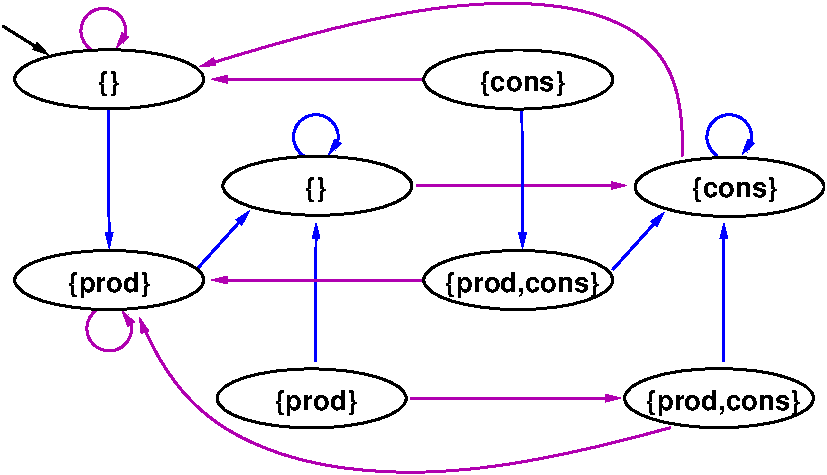
\includegraphics[width=\textwidth]{content/chapter_model_checking/model_checking/images/mutex-krip}
\end{center}

\end{frame}

% ---------------------------------------------------------------------

\begin{frame}{Sequences and trees of valuations}
In \hl{linear-time logic} we consider the possible valuation sequences:

\begin{quote}
z.B.\ \quad \blue{$\emptyset\ \emptyset\ \{{\it prod}\}\ \emptyset\ \{{\it cons}\} \ldots$}
\quad oder \quad
\blue{$\emptyset\ \{{\it prod}\}\ \{{\it prod}\}\ \{{\it prod}\}\ \ldots$}
\end{quote}

\bigskip
In \hl{computation-tree logic} we consider the ``tree-wise unfolding''
   of the Kripke structure:
\begin{center}
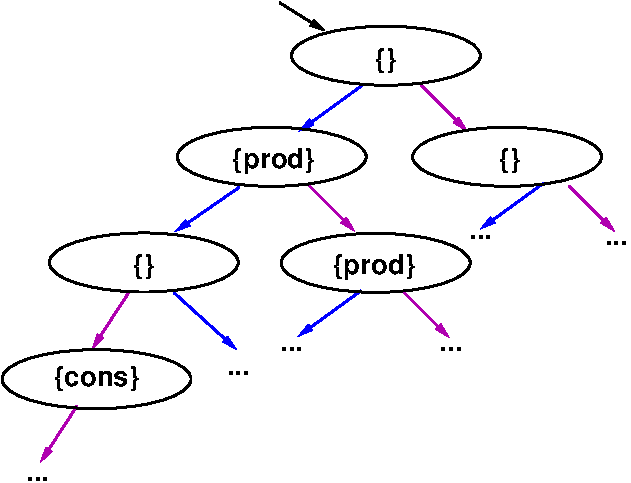
\includegraphics[height=4cm]{content/chapter_model_checking/model_checking/images/mutex-tree}
\end{center}   
\end{frame}

% ---------------------------------------------------------------------

\begin{frame}{Examples of temporal-logic properties}

\hl{``It is never possible that \blue{\it prod}
  and \mag{\it cons} hold at the same time.''}
\begin{quote}
Intuitively, this property holds because no state in which
both \blue{\it prod} and \mag{\it cons} holds is reachable
from the beginning, which can be verified by inspecting the
sequences and trees.
\end{quote}
A property of this form is also called an \hl{invariant}.

\bigskip
\hl{``Whenever something is produced it may be consumed afterwards.''}
\begin{quote}
We may take the view that this property does not hold because of
the following sequence:
\blue{$\emptyset\ \{{\it prod}\}\ \emptyset\ \emptyset\ \emptyset \ldots$}
Thus, something is produced but followed by an infinite loop.
\end{quote}
A property of this form is also called a \hl{reactivity property}.
\end{frame}

% ---------------------------------------------------------------------

\begin{frame}{Fairness}
\begin{itemize}
\item We may also take the view that the second property merely fails
   because of overly simplistic modelling:
\item In the counterexample, only one process is acting, making ``empty''
   steps, while the second process does not do anything.
\item Such a behaviour is usually unrealistic in concurrent systems;
   even if one process may be faster than another and execute multiple
   steps, a ``fair'' scheduler will eventually grant execution time
   to either process.
\item We may therefore wish to exclude such unrealistic (``unfair'') executions
   and only consider ``fair'' ones. In other words, we work under certain
   ``fairness assumptions''.
\item Under a reasonable fairness assumption, the second property holds.
\end{itemize}
\end{frame}

% ---------------------------------------------------------------------

